\section{A taxonomy-tree-based function and join algorithms}

As mentioned in the Introduction and Preliminary, we can extend the SQL language to support IS-A relations. But this is not enough, we next define the similarity of strings based on the taxonomy tree.


\subsection{Similarity with taxonomy tree}


\begin{definition}[Taxonomy Similarity]
Given two taxonomy tree nodes $n_1$ and $n_2$ with their prefix labels $L(n_1)$ and $L(n_2)$, we say the similarity TS($n_1$,$n_2$) is the longest common prefix of  $n_1$ and $n_2$ over the length of the longer path between $n_1$ and $n_2$, that is,  TS($n_1$,$n_2$,$\mathcal{T}$) = $\frac{LCP(L(n_1),L(n_2))}{min(|L(n_1)|,|L(n_2)|)}$. \end{definition}

\smallskip

Note that according to the above definition, if two nodes have the IS-A relations in the taxonomy, then

For example, consider Figure \ref{fig:taxonomyexample}, the similarity between ``\textsf{Seoul}'' and ``\textsf{Suwon}'' is $\frac{3}{4}$= 0.75 (as both countries are in South Korea.), and the the similarity between ``\textsf{Seoul}'' and ``\textsf{Shenzhen}'' is only $\frac{1}{4}$= 0.25 (as two countries are in Asia).

\subsection{Join algorithms}


We would formulate the string similarity join problem and develop the corresponding algorithms. Given two collections of strings $S$ and $T$, a taxonomy tree
$\mathcal{T}$, and a similarity threshold $\theta$, a \textit{string
  similarity join} finds all string pairs $(s, t) \in S \times T$,
such that $TS(s,t,\mathcal{T})$ $>$ $\theta$, where \textit{TS} is
 the taxonomy similarity functions defined above.



Given two collections of strings $S$ and $T$, the baseline join algorithm is the nested-loop join. All string pairs are accessed to determine the IS-A relationships. But this algorithm is obviously not efficient. Therefore, we propose an efficient algorithm.

The key to an efficient, uniform mechanism for set-at-atime
(join-based) matching of query graph patterns is a positional
representation of occurrences of  elements and in the taxonomy database (see, e.g., [6, 7, 27]),
which extends the classic inverted index data structure in information retrieval [22]. We borrow the labeling scheme from XML databases and use the prefix based labels. Structural relationships between tree nodes whose positions
are recorded in this fashion can be determined easily for IS-A relationships.


\begin{figure}[t]
\centering
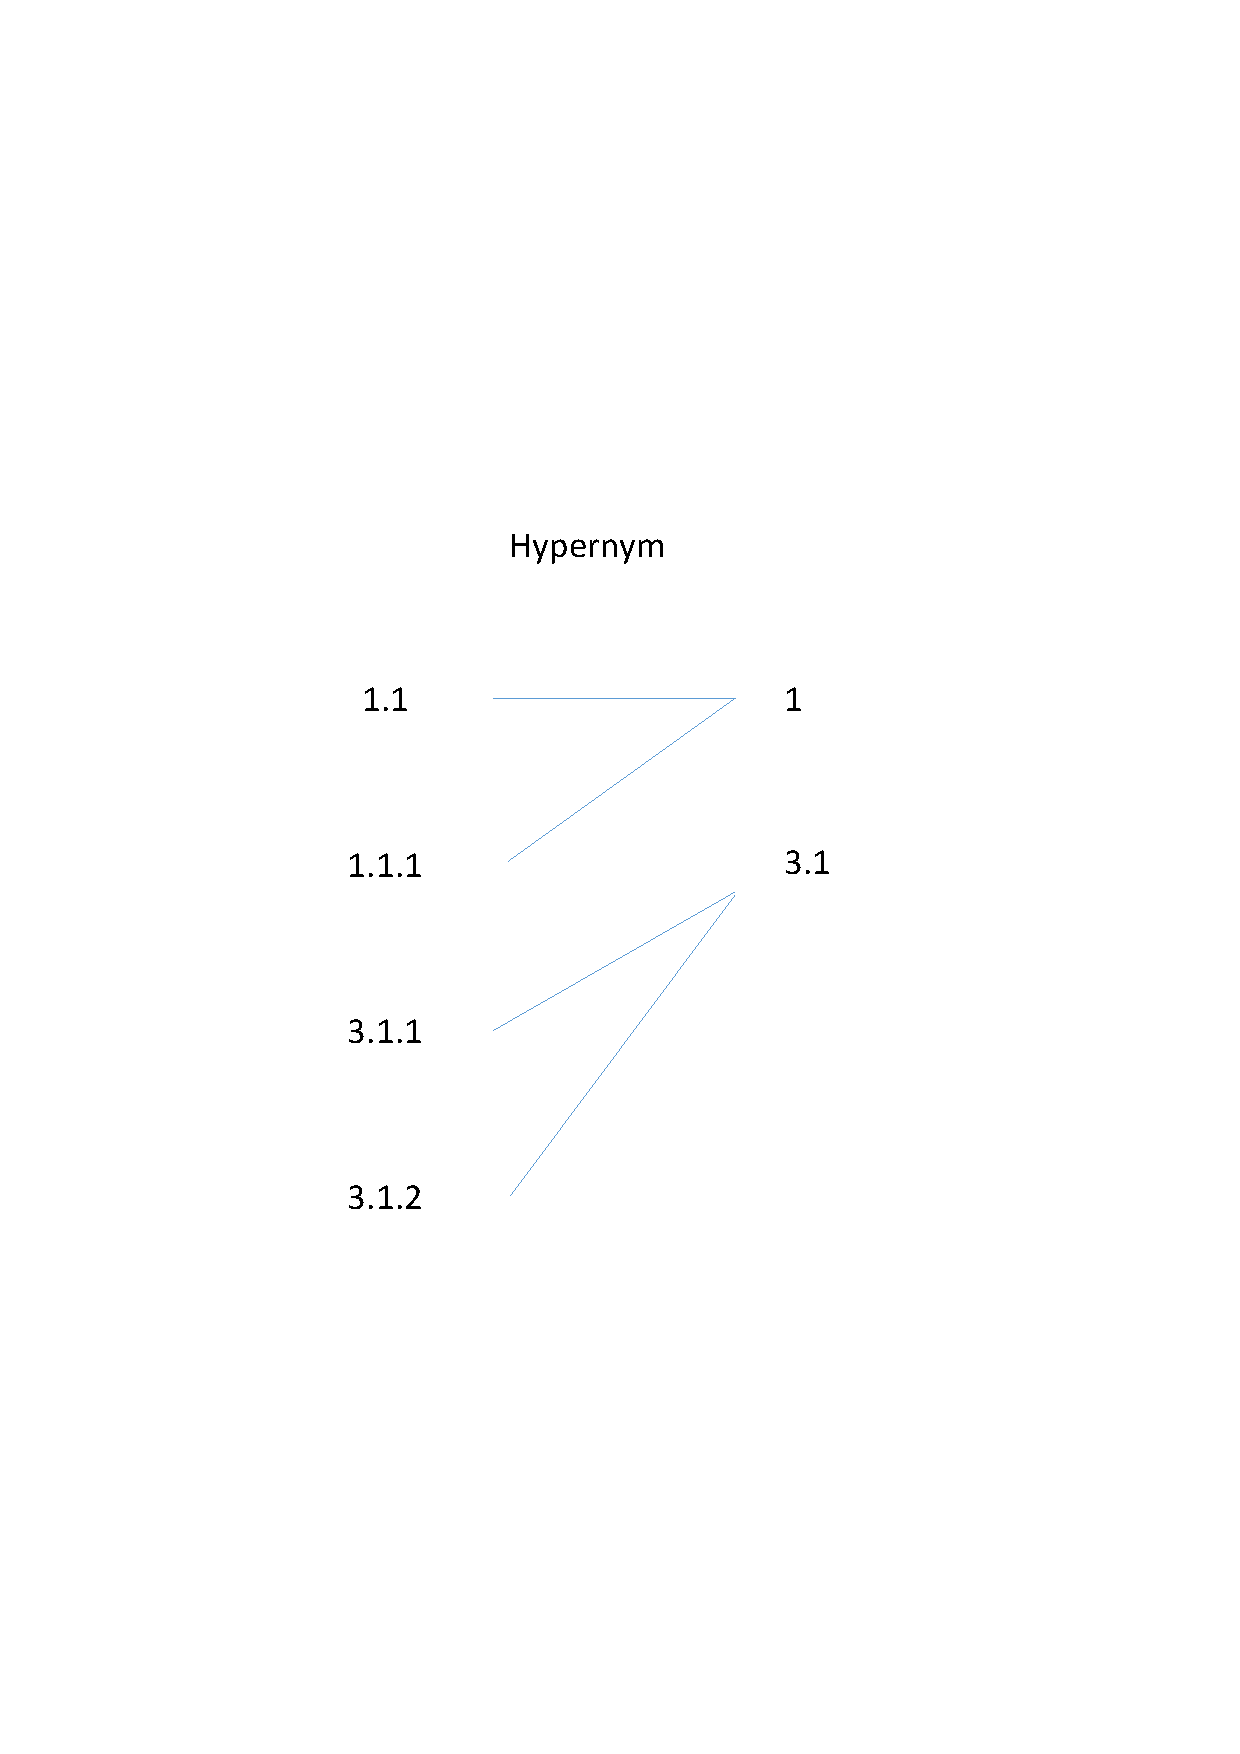
\includegraphics[scale=0.4]{figures/labeljoins}
 \caption{Join inverted lists}
\label{fig:invertedlist}
\end{figure}


%\begin{algorithm}
%{\bf Input}: two strings $s_1$ and $s_2$ \\
%{\bf Output}: four relationships: R=\{Hype, Hypo, Equa and Non\}
%\begin{compactenum}[(1)]
%\item {\bf If} ($s_1 = s_2$ )  {\bf return} Equa;
%\item {\bf If} ($|LCD(s_1)| >$ 1 AND $|LCD(s_2)| >$ 1 )  {\bf return} None;
%\item {\bf Else} {\bf if} ($|LCD(s_1)| =$ 1 AND $|LCD(s_2)| >$ 1 )
%\item \verb"  " {\bf If}  $\forall t \in LCD(s_1)$, $t$ is a hypernym of $LCD(s_2)$
%\item \verb"    " {\bf return} Hype {\bf else} {\bf return} None;
%\item {\bf Else} {\bf if} ($|LCD(s_2)| =$ 1 AND $|LCD(s_1)| >$ 1 )
%\item \verb"  " {\bf If}  $\forall t \in LCD(s_2)$, $t$ is a hypernym of $LCD(s_1)$
%\item  \verb"    " {\bf return} Hypo {\bf else} {\bf return} None;
%\item {\bf Else} /\ *  $|LCD(s_1)| = |LCD(s_2)| = $ 1 */\
%\item  \verb"  " {\bf If}  $LCD(s_1)$ is a hypernym of $LCD(s_2)$  {\bf return} Hype
%\item   \verb"  " {\bf Else if}  $LCD(s_1)$ is a hyponym of $LCD(s_2)$  {\bf return} Hypo
%\item   \verb"  " {\bf Else return} none
%\end{compactenum}
%\caption{Determine the relationship between two strings}
%\label{alg:measure}
%\end{algorithm}





\begin{algorithm}
{\bf Input}: two sets of strings $S_1$ and $S_2$, a taxonomy $\mathcal{T}$, a threshold $\theta$ \\
{\bf Output}: string pairs $(s_1,s_2) \in S_1 \times S_2$, s.t. $TS(s_1, s_2) > \theta$
\begin{compactenum}[(1)]
\item Let $L_s$ and $L_t$ denote the inverted lists for S and T respectively.
\item Let $L$ be the shorted list between $L_s$ and $L_t$.
\item {\bf FOR} EACH element $n$ in $L$ DO
\item ~~~ findTS(n,T,$\theta$);
\item {\bf FOR} EACH join pair ($t_1,t_2$)
\item  Add $t_1.List \times t_2.List$ to R;
\item RETURN $R$
\end{compactenum}
\caption{String joins with taxonomy}
\label{alg:exactjoin}
\end{algorithm}


\begin{algorithm}
{\bf Input}: A node n in T and a threshold $\theta$ \\
{\bf Output}:  pairs $R$ = \{$(n,m) \in L_1 \times L_2$ s.t. $TS(n,m) > \theta$\}
\begin{compactenum}[(1)]
\item FOR EACH i=1 to $|n|$
\item ~~~ $l$ = $\lceil \theta \cdot i \rceil$
\item ~~~ $p$ = $getPrefix(n,l)$
\item ~~~ IF $i < |n|$ THEN
\item ~~~~~~~ Add all nodes with the length $i$ and the prefix $p$ to R;
\item ~~~ ELSE   Add all nodes with the prefix $p$ to R;
\end{compactenum}

%\smallskip
%
%{\bf Function} getMinLabel()
%\begin{compactenum}[(1)]
% \item   ~~~~~~   \textbf{RETURN} min(next($L_{T1}$),next($L_{T2})$) \\
% \end{compactenum}
%
% {\bf Function} getMaxLabel()
%\begin{compactenum}[(1)]
% \item   ~~~~~~   \textbf{RETURN} max(next($L_{T1}$),next($L_{T2})$) \\
% \end{compactenum}


 \caption{findTS(n,T,$\theta$)}
\label{alg:treejoin}
\end{algorithm}


Associated with a collection $T$ there is a list $L_T$. This list contain the positional representation of the taxonomy tree nodes that match strings in the $T$. The nodes in the list are sorted by the lexicographical order. The operation over lists are: Eof, advance, next.


\begin{theorem}  Algorithm \ref{alg:exactjoin} is an optimal algorithm. The computing cost is linear to the sum of the size of the input and output. That is, each output result contribute to the final answer.
\end{theorem}




